\section{Diseño Esquemático y Funcionamiento}

En esta sección se presentan los diagramas que ilustran el diseño arquitectónico y los principales flujos de operación del sistema HTTPS implementado en el proyecto. Cada figura se acompaña de una explicación técnica detallada que facilita la comprensión de los componentes, las interacciones y las implicaciones de seguridad de cada etapa.

\subsection{Arquitectura General del Sistema}
\label{subsec:arquitectura_general}

\begin{figure}[H]
    \centering
    % Cambia el nombre del archivo por el de tu imagen exportada desde mermaid
    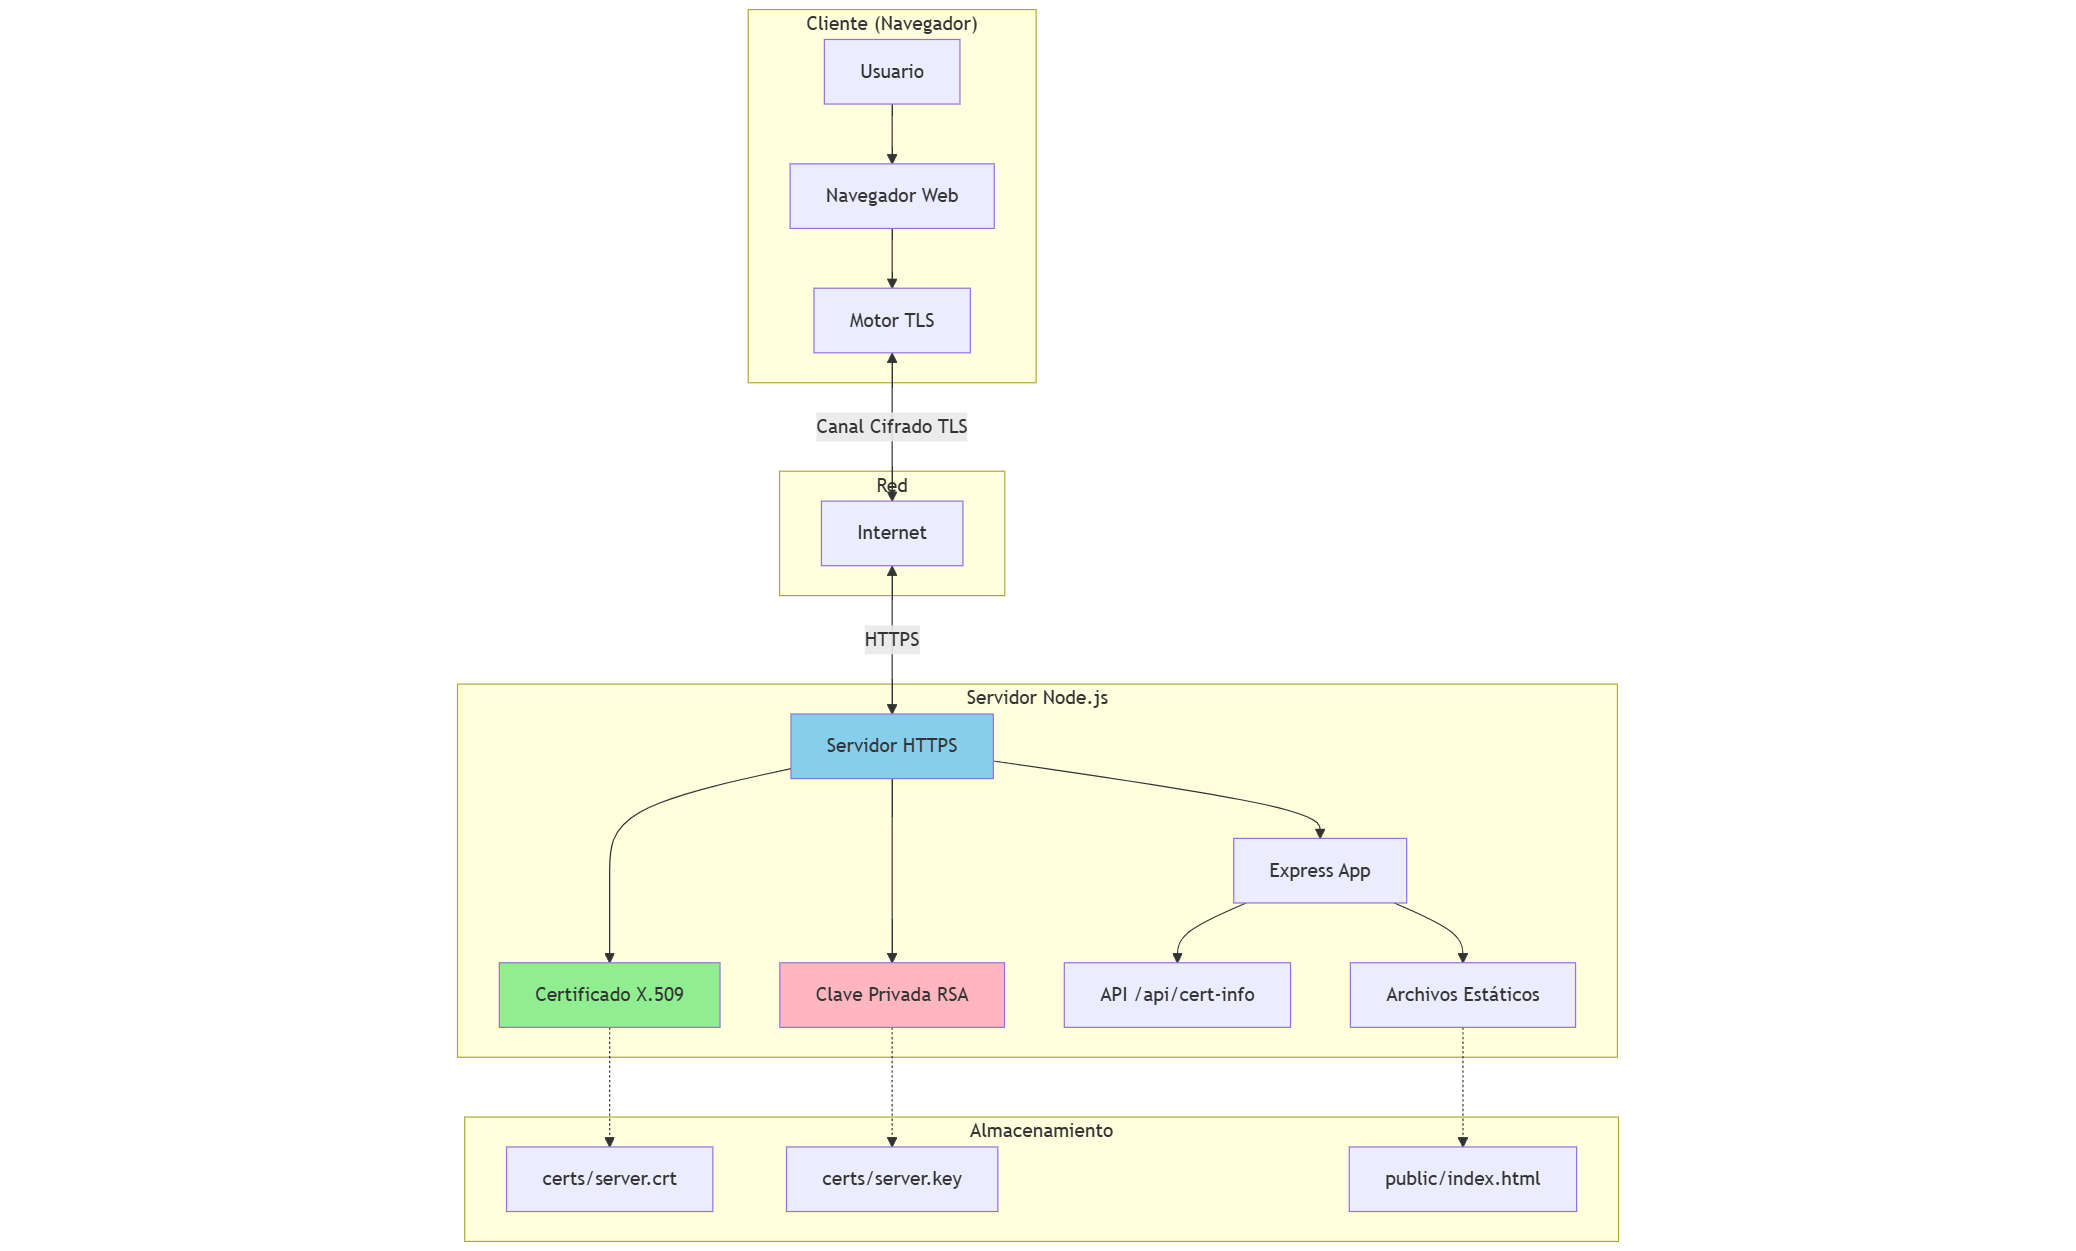
\includegraphics[width=0.9\textwidth]{assets/images/mermaid-diagram-2025-11-29-193228.png}
    \caption{Arquitectura general del sistema: cliente, red, servidor Node.js y almacenamiento de certificados.}
    \label{fig:arquitectura_general}
\end{figure}

\paragraph{Explicación detallada.}  
La figura \ref{fig:arquitectura_general} muestra una visión de alto nivel de los componentes que participan en la provisión de acceso web seguro mediante HTTPS en el entorno del proyecto. Desde la izquierda, el \emph{Cliente (Navegador)} representa el agente que inicia la comunicación —por ejemplo un navegador de escritorio o una aplicación cliente— y que contiene un motor TLS encargado de orquestar el protocolo (negociación de parámetros, verificación de certificados y cifrado/descifrado de datos). El motor TLS actúa como una capa intermedia entre la aplicación (HTTP) y la pila de transporte (TCP/IP), permitiendo que toda la comunicación de la capa de aplicación se beneficie de las garantías criptográficas sin modificar el protocolo HTTP subyacente \cite{rfc8446}.

En el centro se ubica la \emph{Red / Internet}, que representa el canal potencialmente adversarial. Sobre la derecha se encuentra el \emph{Servidor Node.js}, el componente de ejecución que hospeda la aplicación (Express.js) y que expone servicios HTTP sobre un socket TLS (HTTPS). En él se distinguen claramente dos artefactos críticos: el \textbf{Certificado X.509} (archivo \texttt{certs/server.crt}) y la \textbf{Clave Privada RSA} (archivo \texttt{certs/server.key}). El correcto almacenamiento, acceso y permisos de estos ficheros son esenciales: la clave privada debe protegerse con controles de acceso estrictos y, preferiblemente, con cifrado en reposo y políticas de rotación en entornos productivos \cite{rfc5280}.

La sección de \emph{Almacenamiento} indica la localización física/estructural de los artefactos (certificado, clave privada, recursos estáticos). En un despliegue real, este almacenamiento puede estar respaldado por módulos HSM o servicios de gestión de claves para incrementar la seguridad y minimizar el riesgo de exposición de la llave privada. Desde el punto de vista funcional, la arquitectura enfatiza la separación de responsabilidades: el servidor HTTPS se encarga del manejo del canal seguro y de proporcionar una interfaz a la aplicación (Express) que permanece, conceptualmente, agnóstica respecto al cifrado de transporte.

\bigskip

\subsection{Flujo de Comunicación Completo (Handshakes y Tráfico)}
\label{subsec:flujo_comunicacion}

\begin{figure}[H]
    \centering
    % Cambia el nombre del archivo por el de tu imagen exportada desde mermaid
    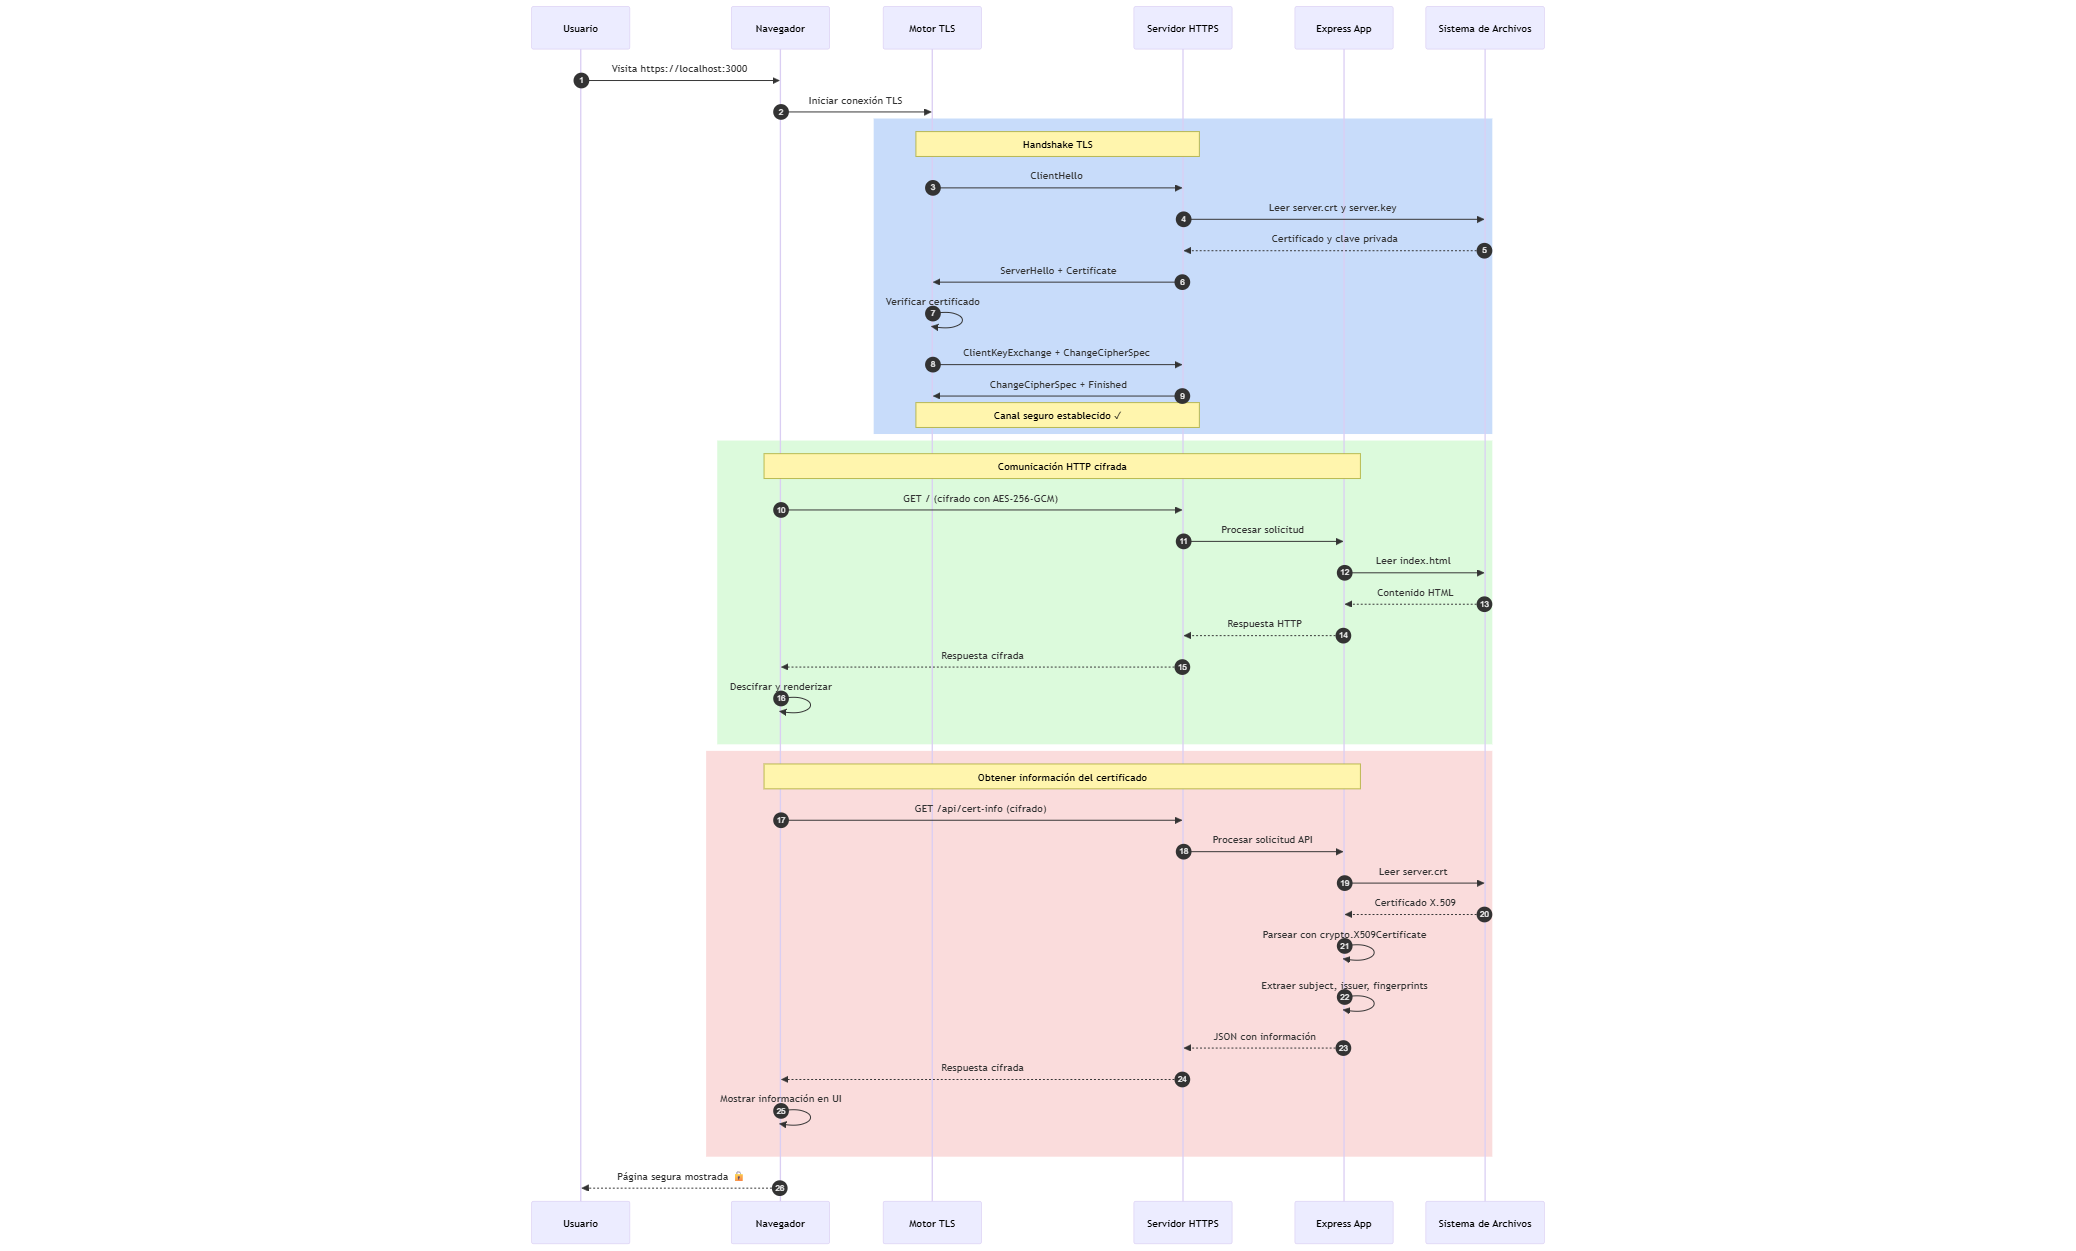
\includegraphics[width=0.95\textwidth]{assets/images/mermaid-diagram-2025-11-29-193405.png}
    \caption{Flujo completo de comunicación: Handshake TLS, establecimiento del canal seguro y tráfico de aplicación cifrado.}
    \label{fig:flujo_comunicacion}
\end{figure}

\paragraph{Explicación detallada.}  
La figura \ref{fig:flujo_comunicacion} descompone cronológicamente las interacciones que se producen desde que el usuario solicita la URL hasta que el navegador renderiza la página segura. El proceso puede resumirse en tres fases principales:

\begin{enumerate}
    \item \textbf{Establecimiento del handshake TLS:} El cliente envía un \texttt{ClientHello} que contiene las versiones TLS soportadas, cipher suites y extensiones relevantes (SNI, ALPN, etc.). El servidor responde con \texttt{ServerHello}, seleccionando los parámetros de cifrado y proporcionando su certificado X.509 en el mensaje \texttt{Certificate}. El servidor también realiza la demostración de posesión de la clave privada mediante \texttt{CertificateVerify}, permitiendo al cliente validar la autenticidad del servidor. TLS 1.3 reduce el número de intercambios y cifra gran parte del handshake para mejorar privacidad y rendimiento \cite{rfc8446, bhargavan2014}.
    \item \textbf{Negociación de claves y establecimiento del canal seguro:} Tras la verificación del certificado y la negociación de parámetros, se generan claves de sesión efímeras (p. ej. mediante ECDHE) que garantizan \emph{Perfect Forward Secrecy}. A partir de ese momento, el \emph{Record Protocol} utiliza algoritmos AEAD (AES-GCM o ChaCha20-Poly1305) para cifrar y autenticar los registros que transportan los mensajes HTTP \cite{rfc7525}.
    \item \textbf{Intercambio de datos de aplicación y gestión de información adicional:} Con el canal seguro establecido, el navegador realiza la petición HTTP (por ejemplo \texttt{GET /}) y el servidor responde con contenido estático o dinámico (páginas, APIs). Notar que las comprobaciones adicionales, como la verificación de estado del certificado (OCSP/OCSP Stapling) o la política HSTS, se evalúan conforme a las necesidades de seguridad del servicio \cite{liu2015, helme2024}.
\end{enumerate}

Desde la perspectiva de auditoría y pruebas, cada una de estas fases puede ser instrumentada y registrada (logs de handshake, huellas del certificado, pruebas con \texttt{curl} o análisis con \texttt{testssl.sh}) para verificar la conformidad del despliegue con las recomendaciones operacionales y los requisitos de seguridad académicos \cite{rfc7525}.

\bigskip

\subsection{Proceso de Generación de Certificados}
\label{subsec:generacion_certificados}

\begin{figure}[H]
    \centering
    % Cambia el nombre del archivo por el de tu imagen exportada desde mermaid
    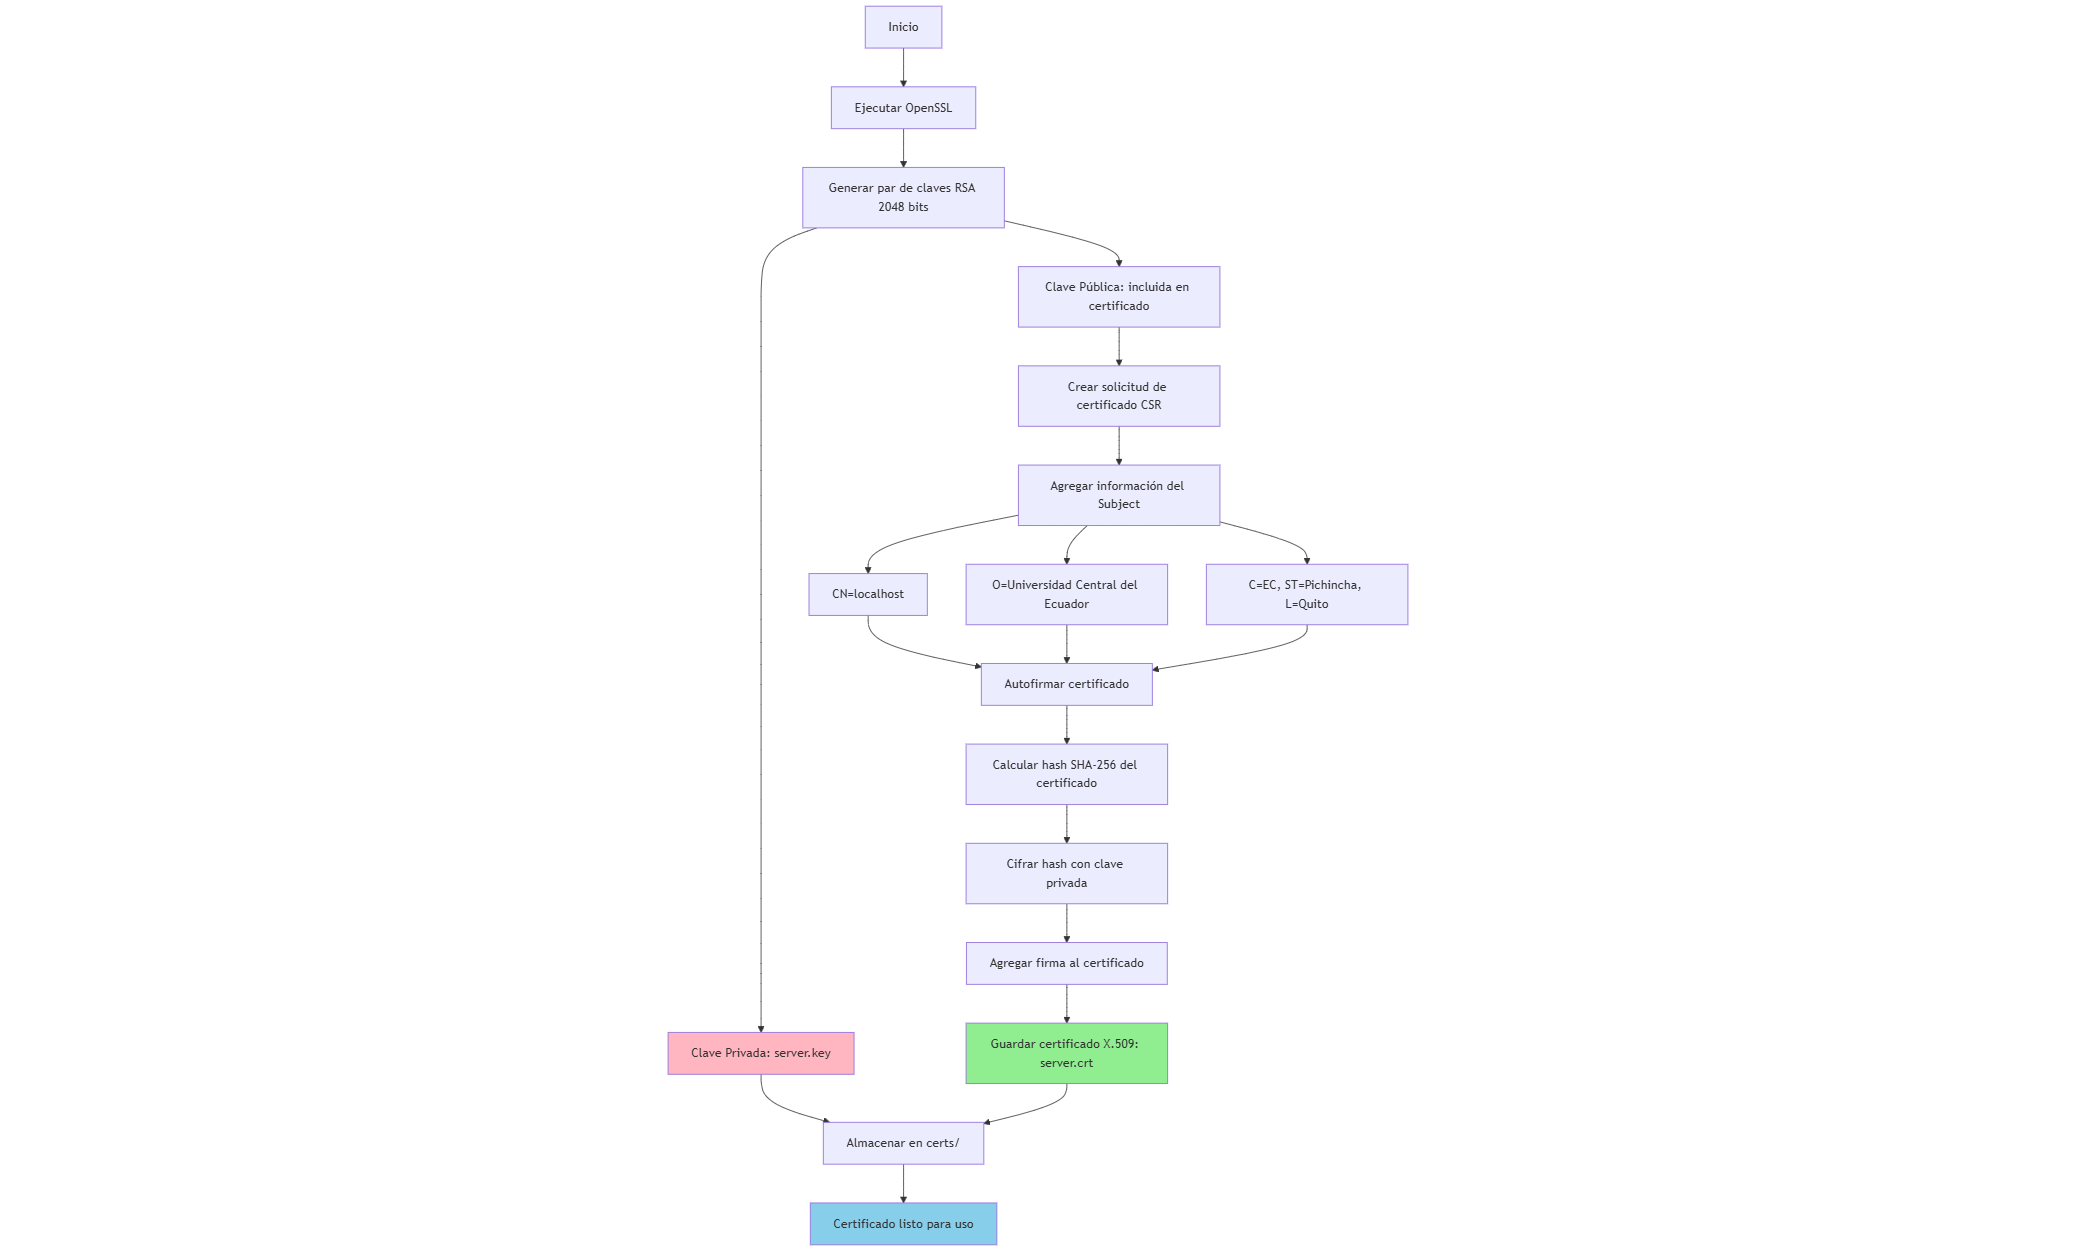
\includegraphics[width=0.75\textwidth]{assets/images/mermaid-diagram-2025-11-29-193526.png}
    \caption{Proceso de generación de certificados X.509 autofirmados mediante OpenSSL (par de claves RSA, CSR, autofirma y almacenamiento).}
    \label{fig:proceso_certificados}
\end{figure}

\paragraph{Explicación detallada.}  
La figura \ref{fig:proceso_certificados} describe el flujo lógico para la generación de un certificado X.509 autofirmado utilizado en el entorno de laboratorio. El proceso consta de los pasos siguientes:

\begin{enumerate}
    \item \textbf{Generación del par de claves (clave privada y clave pública):} Mediante OpenSSL se crea un par RSA (p. ej. 2048 o 4096 bits) o una clave basada en curvas elípticas (p. ej. Curve25519). La clave privada se escribe en un fichero seguro (\texttt{server.key}) y su correlato público será parte de la CSR (Certificate Signing Request) o del certificado final \cite{rfc5280}.
    \item \textbf{Creación de la CSR (Solicitud de Firma de Certificado):} La CSR contiene la información de identidad (CN, O, OU, L, ST, C) y la clave pública. En un entorno de producción, esta CSR se envía a una CA para validación; en el laboratorio se puede proceder a la autofirma.
    \item \textbf{Autofirma del certificado:} En la autofirma, el emisor y sujeto son la misma entidad; por tanto, el certificado resultante es firmado con la propia clave privada y carece de la confianza automática que una CA pública proporciona a navegadores y sistemas clientes. Aun así, constituye una herramienta válida para pruebas y enseñanza, permitiendo analizar el contenido del certificado y las firmas digitales que lo componen \cite{rfc5280}.
    \item \textbf{Cálculo y adición de la firma:} El certificado incluye una firma digital calculada mediante un algoritmo como \texttt{sha256WithRSAEncryption} que cifra el hash (SHA-256) del TBS (To-Be-Signed) certificate con la clave privada del emisor.
    \item \textbf{Almacenamiento y despliegue:} Finalmente, el certificado (\texttt{server.crt}) y la clave privada (\texttt{server.key}) se guardan en el directorio de certificados del servidor y se referencian en la configuración de la instancia HTTPS para su carga en tiempo de arranque.
\end{enumerate}

Es importante subrayar las diferencias entre certificados autofirmados y certificados emitidos por CA: los segundos permiten establecer una cadena de confianza globalmente aceptada por los navegadores; los primeros requieren que el cliente añada explícitamente la CA raíz (o se acepte la excepción) y por tanto son apropiados únicamente para entornos controlados de laboratorio \cite{liu2015}.

\bigskip

\subsection{Estructura de Datos del Certificado X.509}
\label{subsec:estructura_certificado}

\begin{figure}[H]
    \centering
    % Cambia el nombre del archivo por el de tu imagen exportada desde mermaid
    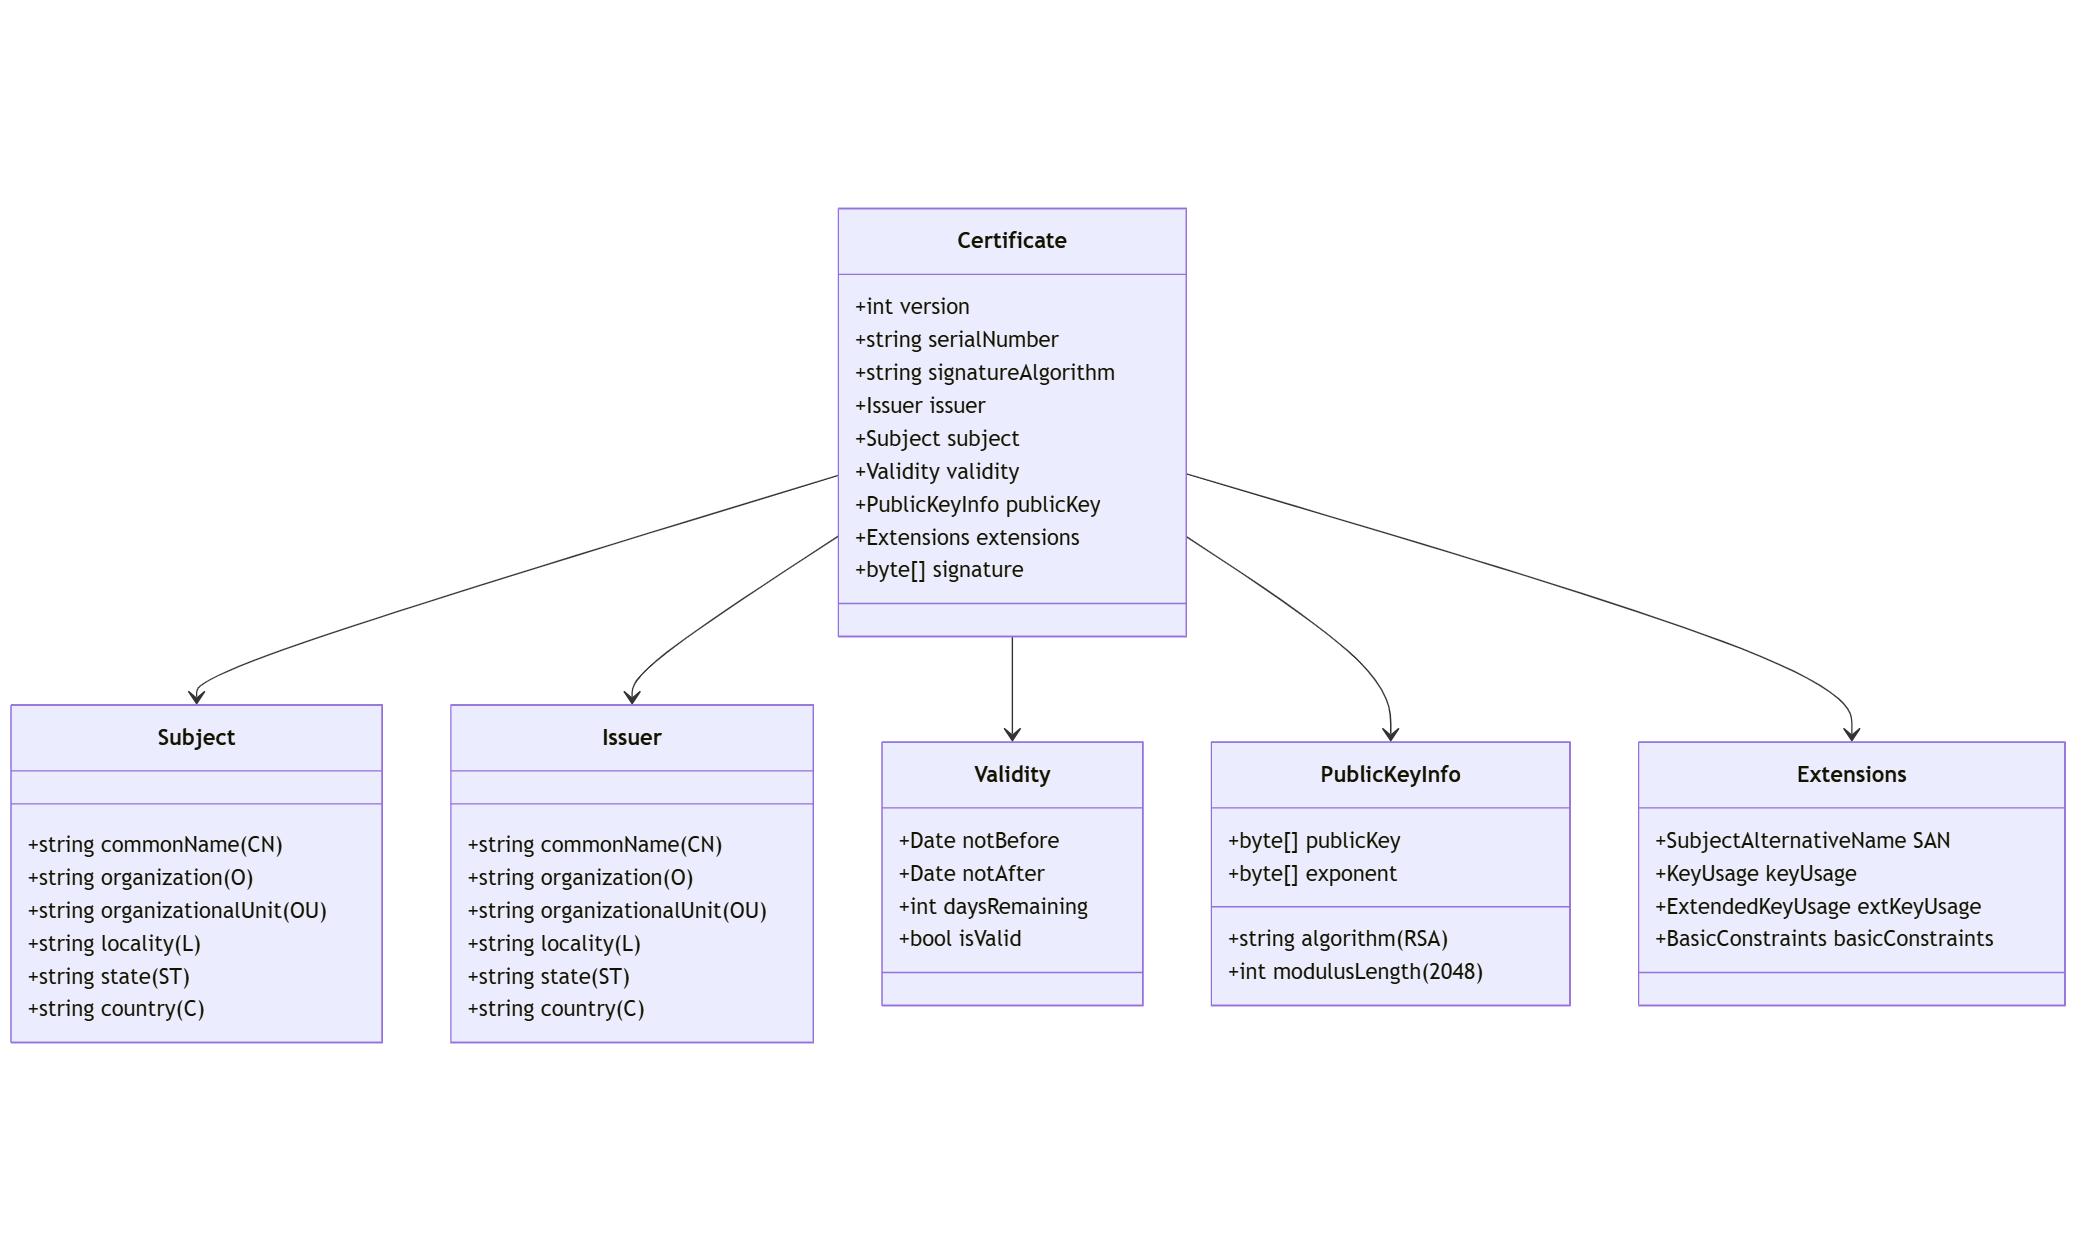
\includegraphics[width=0.85\textwidth]{assets/images/mermaid-diagram-2025-11-29-193726.png}
    \caption{Estructura de datos de un certificado X.509 v3: campos básicos, validez, clave pública y extensiones.}
    \label{fig:estructura_x509}
\end{figure}

\paragraph{Explicación detallada.}  
La figura \ref{fig:estructura_x509} desglosa los componentes esenciales de un certificado X.509 versión 3. Cada campo cumple una función específica en la identificación y autorización criptográfica:

\begin{description}
    \item[Version y Serial Number:] Identificadores del formato y del ejemplar del certificado, usados para la gestión y revocación.
    \item[Signature Algorithm:] Algoritmo empleado para la firma del certificado (p. ej. \texttt{sha256WithRSAEncryption}). La seguridad de este campo depende tanto del algoritmo como del tamaño de la clave subyacente \cite{rfc5280}.
    \item[Issuer y Subject:] Identificadores de la entidad emisora y del titular (titular = subject). En una CA legítima, la cadena de confianza se construye mediante la relación Issuer $\rightarrow$ Subject a través de firmas encadenadas.
    \item[Validity (notBefore / notAfter):] Período de validez del certificado. Exceder este período hará que el certificado sea inválido para la mayoría de clientes.
    \item[Subject Public Key Info:] Contiene la clave pública y parámetros asociados (algoritmo, longitud de clave). Esta clave es la base para la verificación de firmas y, en combinación con protocolos de intercambio, para la protección de sesiones.
    \item[Extensions:] Conjunto de extensiones X.509v3 (SAN, KeyUsage, ExtendedKeyUsage, BasicConstraints, etc.) que proporcionan metadatos críticos para el uso correcto del certificado. Por ejemplo, SAN (Subject Alternative Name) define dominios alternativos válidos para el certificado y es fundamental para la validación de nombres por parte de navegadores.
    \item[Signature:] Firma criptográfica del TBS (To-Be-Signed) certificate generada por la entidad emisora. Su verificación es el paso clave de la validación de confianza en TLS \cite{rfc5280}.
\end{description}

Comprender la estructura interna del certificado es imprescindible para interpretar resultados de herramientas de análisis (por ejemplo \texttt{openssl x509 -text -noout -in server.crt}) y para diseñar políticas de emisión, rotación y revocación de certificados en ambientes reales \cite{liu2015}.

\bigskip

\subsection{Implementación en Node.js: Integración y Componentes}
\label{subsec:implementacion_nodejs}

\begin{figure}[H]
    \centering
    % Cambia el nombre del archivo por el de tu imagen exportada desde mermaid
    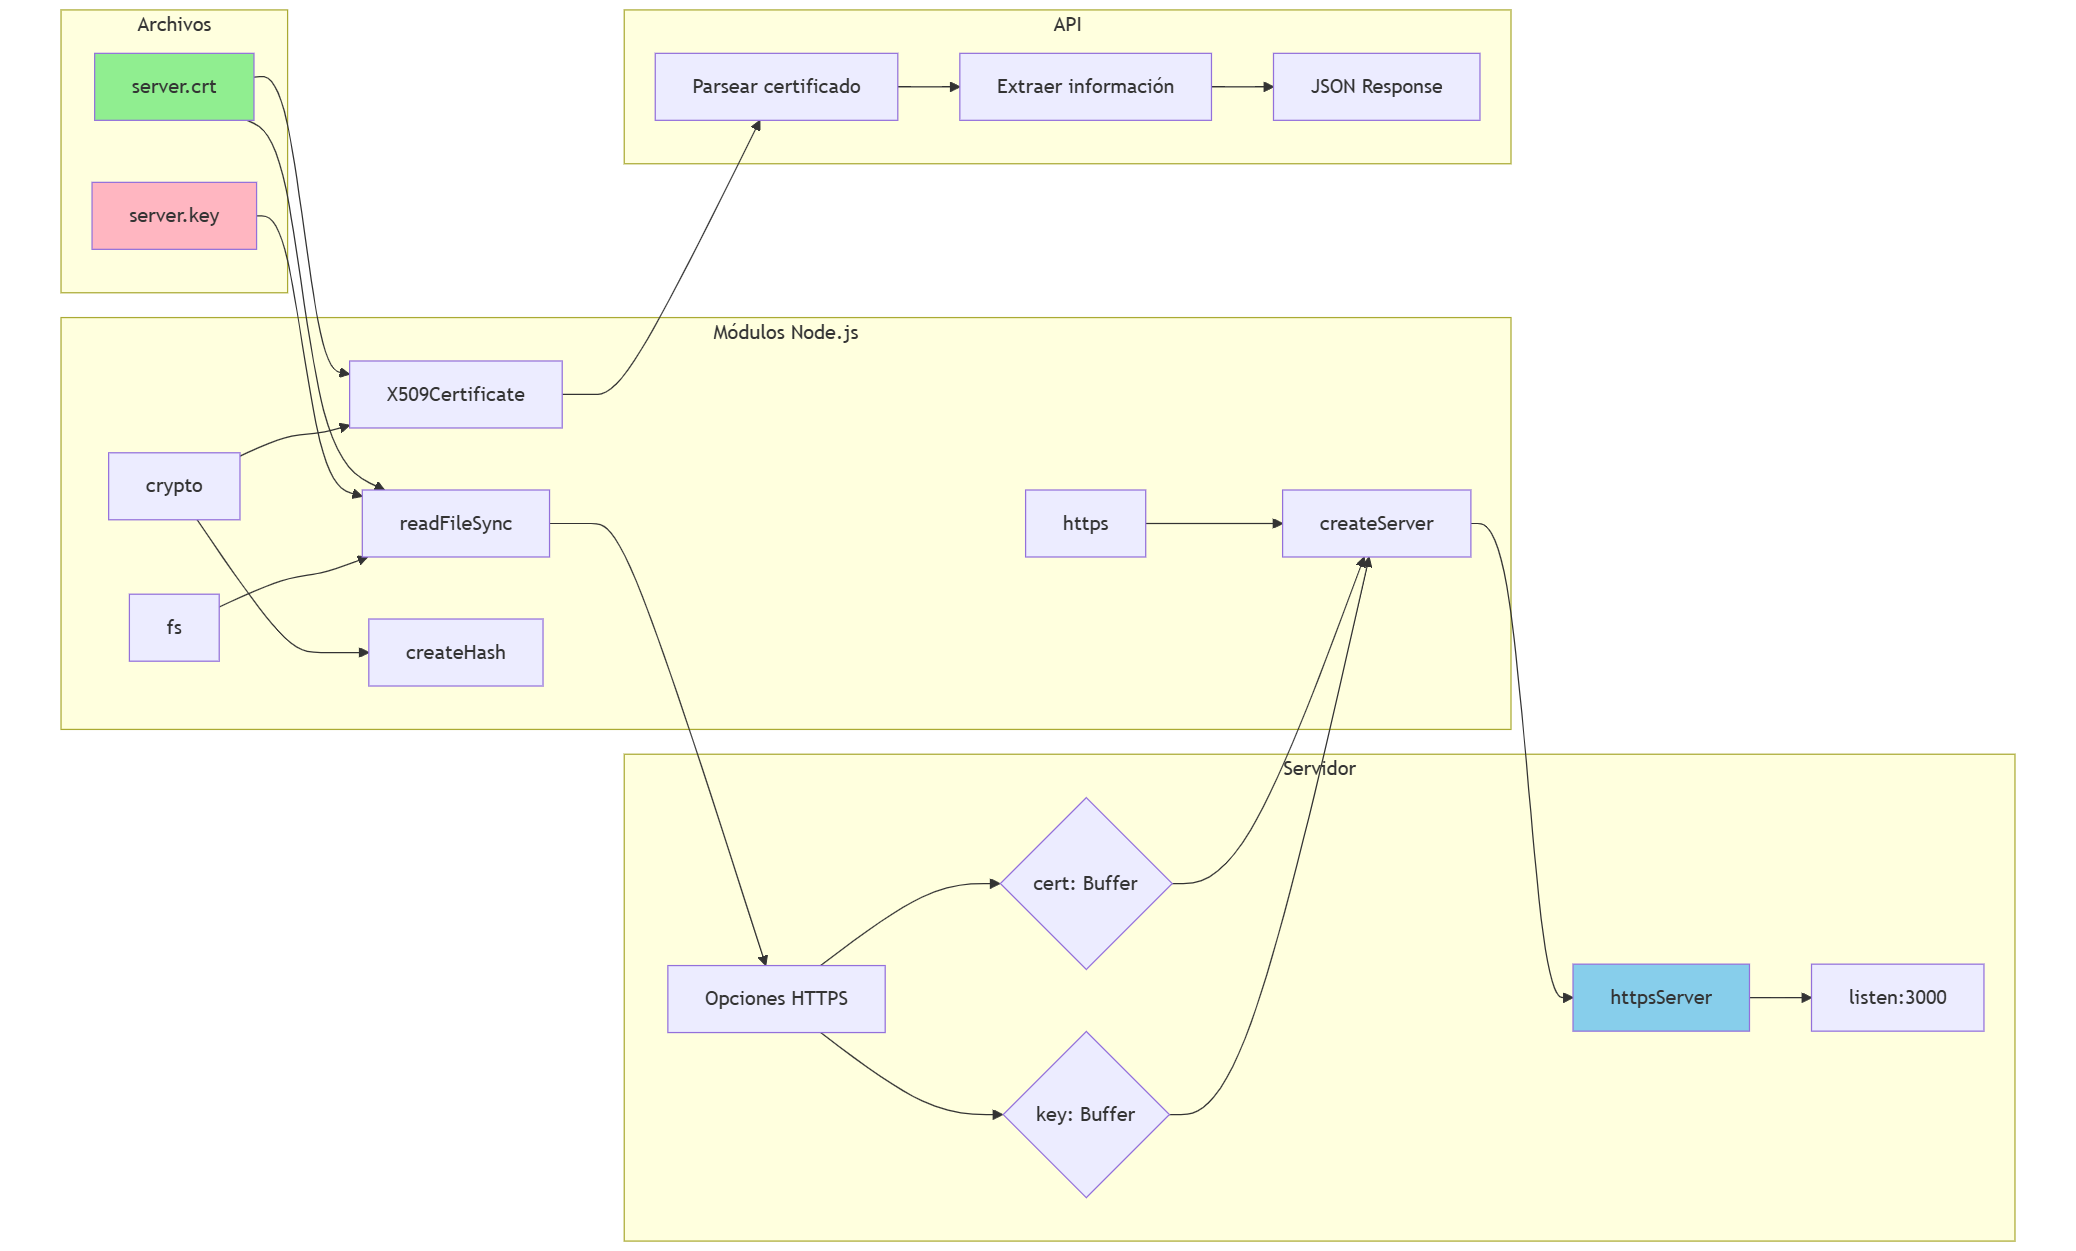
\includegraphics[width=0.9\textwidth]{assets/images/mermaid-diagram-2025-11-29-193820.png}
    \caption{Componentes Node.js implicados en la creación de un servidor HTTPS: módulos, archivos y flujo de carga.}
    \label{fig:implementacion_nodejs}
\end{figure}

\paragraph{Explicación detallada.}  
La figura \ref{fig:implementacion_nodejs} ilustra la relación entre los módulos nativos de Node.js (\texttt{https}, \texttt{fs}, \texttt{crypto}), los archivos de certificados en disco y la instancia del servidor que escucha en un puerto seguro (ej. 3000 para desarrollo). El flujo de arranque típico es:

\begin{enumerate}
    \item \textbf{Lectura de artefactos criptográficos:} El servidor, durante su inicialización, emplea \texttt{fs.readFileSync()} para cargar \texttt{server.key} y \texttt{server.crt} en buffers de memoria. Es recomendable proteger estos archivos mediante permisos de sistema operativo y, si es viable, cargarlos desde un HSM o un almacén cifrado.
    \item \textbf{Configuración de opciones HTTPS:} Se construye un objeto de opciones con las propiedades \texttt{key}, \texttt{cert} y, opcionalmente, \texttt{ca}, \texttt{honorCipherOrder} y parámetros de curvas elípticas preferidas. Estos parámetros determinan la política criptográfica del servidor y deben alinearse con las recomendaciones de RFC y las mejores prácticas (por ejemplo, preferir ECDHE y AEAD).
    \item \textbf{Creación del servidor HTTPS:} Con \texttt{https.createServer(options, app)} se instancia el servidor que delega en \texttt{app} (Express) el manejo de rutas y lógica de negocio. El servidor expone tanto recursos estáticos como endpoints API (p. ej. \texttt{/api/cert-info}) que pueden devolver metadatos del certificado para fines de diagnóstico.
    \item \textbf{Operación en tiempo de ejecución:} Una vez iniciado, el servidor acepta conexiones TLS entrantes, realiza el handshake, negocia cipher suites y atiende peticiones cifradas. Es importante instrumentar el servidor con métricas y logs que permitan identificar fallos de handshakes, intentos de conexión rechazados o advertencias relativas a suites inseguras.
\end{enumerate}

Desde la perspectiva de seguridad operativa, se enfatiza la necesidad de:

\begin{itemize}
    \item Minimizar la exposición de la clave privada y aplicar rotación periódica.
    \item Configurar políticas claras de cipher suites y deshabilitar suites obsoletas.
    \item Implementar OCSP Stapling, HSTS y cabeceras de seguridad HTTP adicionales para reducir vectores de ataque de downgrade y mejora la privacidad del cliente \cite{rfc7525, liu2015}.
\end{itemize}

\bigskip

\noindent\textbf{Notas finales:} Las figuras y sus explicaciones constituyen un marco detallado que permite tanto al lector académico como al practicante reproducir, analizar y evaluar la implementación de HTTPS en un entorno controlado. Para despliegues en producción se recomiendan controles adicionales (HSM, auditoría de claves, gestión de revocación a escala) y la supervisión continuada de vulnerabilidades reportadas (CVE/NVD) que puedan afectar a las bibliotecas criptográficas y al propio servidor.
